\subsubsection{UC18 - Rimozione funzione}
\begin{figure}[h]
	\centering
	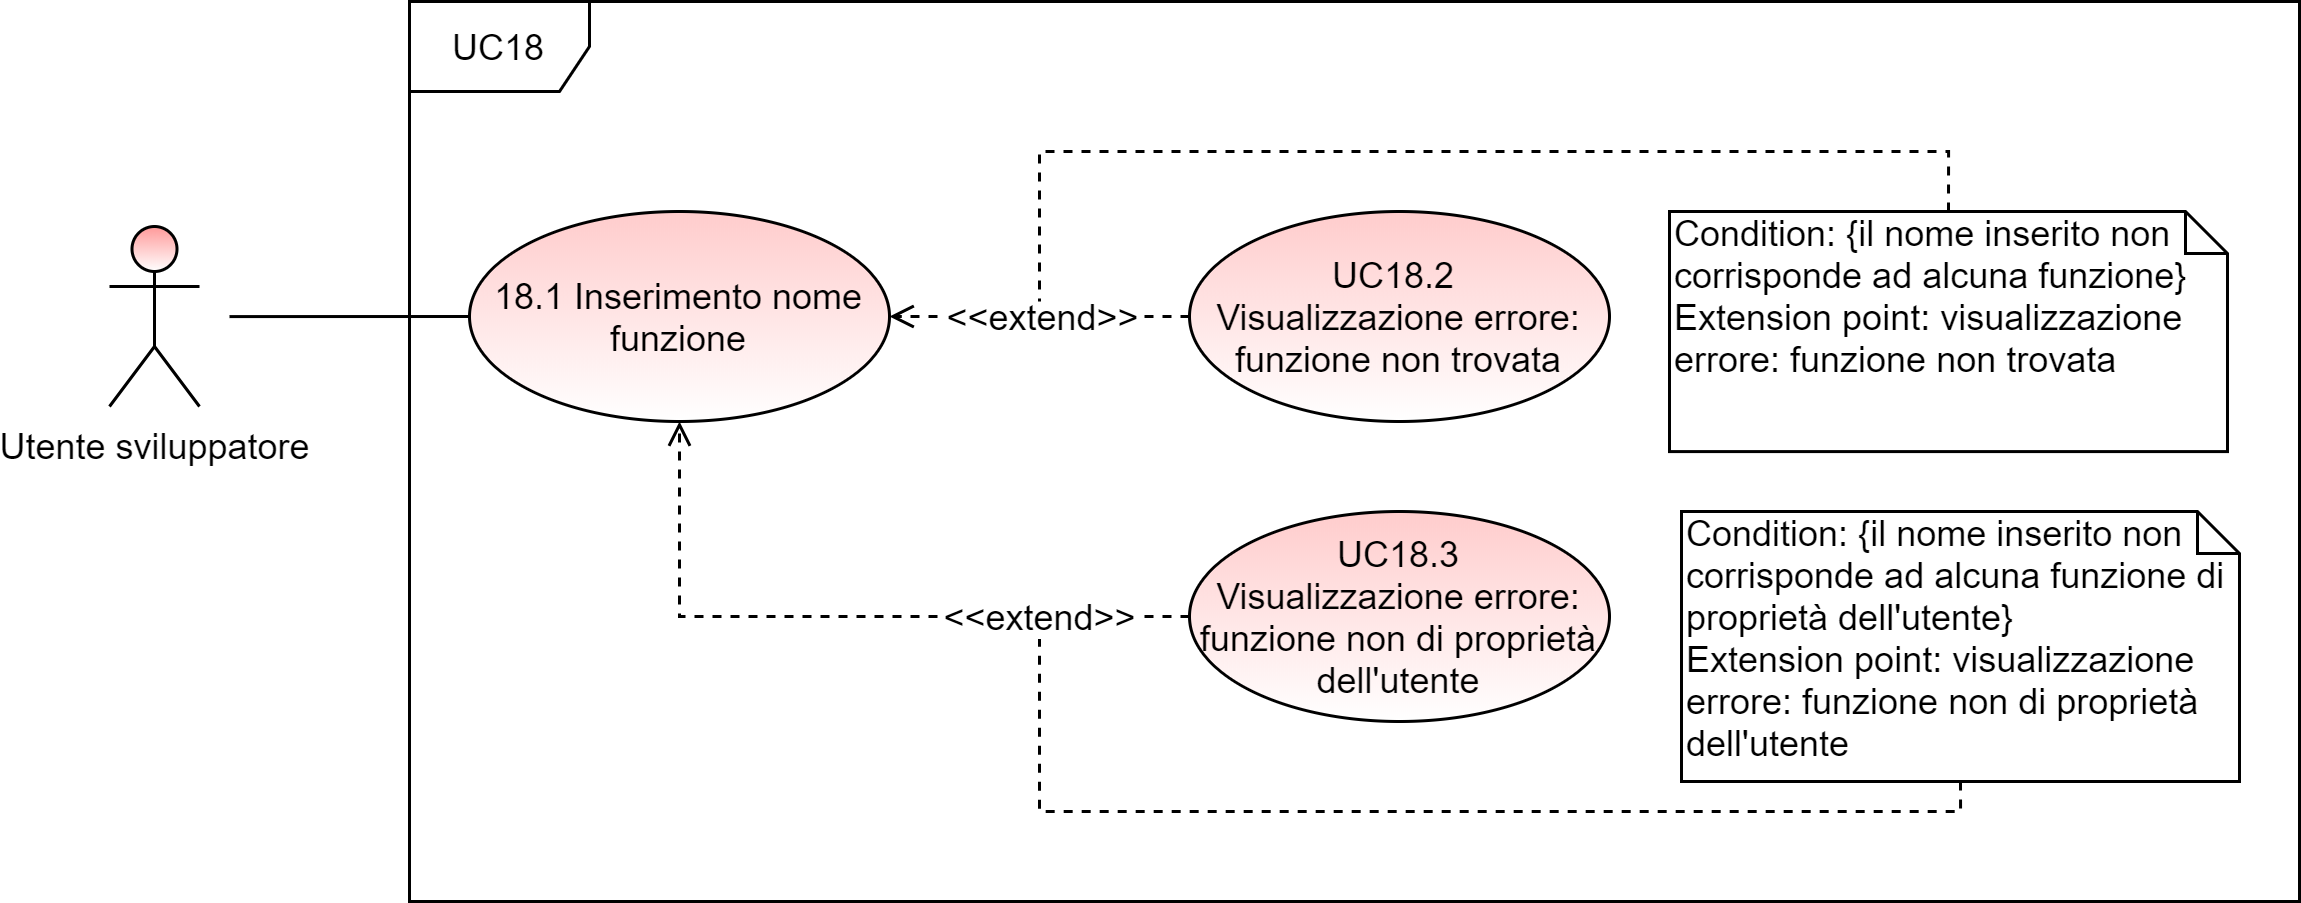
\includegraphics[scale=\ucs]{./res/img/UC18.png}
	\caption {UC18 - Rimozione funzione}
\end{figure}
\begin{itemize}
	\item \textbf{Attori primari:} \us{};
	\item \textbf{Attori secondari:} \re{};
	\item \textbf{Descrizione:} attraverso l’utilizzo del comando \delete{} l’utente può procedere alla rimozione di una funzione;  
	\item \textbf{Scenario principale:} 
	\begin{itemize}
		\item l’utente inserisce il comando \delete{} seguito dal nome della funzione da rimuovere; 
		\item la funzione viene rimossa con successo. 
	\end{itemize}
	\item \textbf{Precondizione:} l’utente vuole rimuovere una funzione dal sistema;  
	\item \textbf{Postcondizione:} la funzione è stata rimossa con successo dal sistema.
\end{itemize}